\documentclass[man,floatsintext]{apa6}
\usepackage{lmodern}
\usepackage{amssymb,amsmath}
\usepackage{ifxetex,ifluatex}
\usepackage{fixltx2e} % provides \textsubscript
\ifnum 0\ifxetex 1\fi\ifluatex 1\fi=0 % if pdftex
  \usepackage[T1]{fontenc}
  \usepackage[utf8]{inputenc}
\else % if luatex or xelatex
  \ifxetex
    \usepackage{mathspec}
  \else
    \usepackage{fontspec}
  \fi
  \defaultfontfeatures{Ligatures=TeX,Scale=MatchLowercase}
\fi
% use upquote if available, for straight quotes in verbatim environments
\IfFileExists{upquote.sty}{\usepackage{upquote}}{}
% use microtype if available
\IfFileExists{microtype.sty}{%
\usepackage{microtype}
\UseMicrotypeSet[protrusion]{basicmath} % disable protrusion for tt fonts
}{}
\usepackage{hyperref}
\hypersetup{unicode=true,
            pdftitle={Language use shapes cultural stereotypes: Large scale evidence from gender},
            pdfauthor={Molly Lewis~\& Gary Lupyan},
            pdfkeywords={cultural norms, implicit association task (IAT), gender},
            pdfborder={0 0 0},
            breaklinks=true}
\urlstyle{same}  % don't use monospace font for urls
\usepackage{graphicx,grffile}
\makeatletter
\def\maxwidth{\ifdim\Gin@nat@width>\linewidth\linewidth\else\Gin@nat@width\fi}
\def\maxheight{\ifdim\Gin@nat@height>\textheight\textheight\else\Gin@nat@height\fi}
\makeatother
% Scale images if necessary, so that they will not overflow the page
% margins by default, and it is still possible to overwrite the defaults
% using explicit options in \includegraphics[width, height, ...]{}
\setkeys{Gin}{width=\maxwidth,height=\maxheight,keepaspectratio}
\IfFileExists{parskip.sty}{%
\usepackage{parskip}
}{% else
\setlength{\parindent}{0pt}
\setlength{\parskip}{6pt plus 2pt minus 1pt}
}
\setlength{\emergencystretch}{3em}  % prevent overfull lines
\providecommand{\tightlist}{%
  \setlength{\itemsep}{0pt}\setlength{\parskip}{0pt}}
\setcounter{secnumdepth}{0}
% Redefines (sub)paragraphs to behave more like sections
\ifx\paragraph\undefined\else
\let\oldparagraph\paragraph
\renewcommand{\paragraph}[1]{\oldparagraph{#1}\mbox{}}
\fi
\ifx\subparagraph\undefined\else
\let\oldsubparagraph\subparagraph
\renewcommand{\subparagraph}[1]{\oldsubparagraph{#1}\mbox{}}
\fi

%%% Use protect on footnotes to avoid problems with footnotes in titles
\let\rmarkdownfootnote\footnote%
\def\footnote{\protect\rmarkdownfootnote}


  \title{Language use shapes cultural stereotypes: Large scale evidence from
gender}
    \author{Molly Lewis\textsuperscript{1,2}~\& Gary Lupyan\textsuperscript{1}}
    \date{}
  
\shorttitle{Language use shapes cultural stereotypes}
\affiliation{
\vspace{0.5cm}
\textsuperscript{1} University of Wisconsin-Madison\\\textsuperscript{2} University of Chicago}
\keywords{cultural norms, implicit association task (IAT), gender\newline\indent Word count: X}
\usepackage{csquotes}
\usepackage{upgreek}
\captionsetup{font=singlespacing,justification=justified}

\usepackage{longtable}
\usepackage{lscape}
\usepackage{multirow}
\usepackage{tabularx}
\usepackage[flushleft]{threeparttable}
\usepackage{threeparttablex}

\newenvironment{lltable}{\begin{landscape}\begin{center}\begin{ThreePartTable}}{\end{ThreePartTable}\end{center}\end{landscape}}

\makeatletter
\newcommand\LastLTentrywidth{1em}
\newlength\longtablewidth
\setlength{\longtablewidth}{1in}
\newcommand{\getlongtablewidth}{\begingroup \ifcsname LT@\roman{LT@tables}\endcsname \global\longtablewidth=0pt \renewcommand{\LT@entry}[2]{\global\advance\longtablewidth by ##2\relax\gdef\LastLTentrywidth{##2}}\@nameuse{LT@\roman{LT@tables}} \fi \endgroup}



\authornote{Portions of this manuscript appeared in Lewis \&
Lupyan, 2018, Cog. Sci Proceedings.

Correspondence concerning this article should be addressed to Molly
Lewis, . E-mail:
\href{mailto:mollyllewis@gmail.com}{\nolinkurl{mollyllewis@gmail.com}}}

\abstract{
this is an abstract


}

\usepackage{amsthm}
\newtheorem{theorem}{Theorem}[section]
\newtheorem{lemma}{Lemma}[section]
\theoremstyle{definition}
\newtheorem{definition}{Definition}[section]
\newtheorem{corollary}{Corollary}[section]
\newtheorem{proposition}{Proposition}[section]
\theoremstyle{definition}
\newtheorem{example}{Example}[section]
\theoremstyle{definition}
\newtheorem{exercise}{Exercise}[section]
\theoremstyle{remark}
\newtheorem*{remark}{Remark}
\newtheorem*{solution}{Solution}
\begin{document}
\maketitle

\section{Introduction}\label{introduction}

By the time they are two years old, children have already begun to
acquire the gender stereotypes in their culture (Gelman, Taylor, Nguyen,
Leaper, \& Bigler, 2004). This finding is concerning given evidence that
children's conceptualizations of gender can have undesirable real-world
consequences. For example, in one study, girls, compared to boys, were
less likely to think that girls are \enquote{brilliant} and also less
likely to choose activities that were described as for \enquote{children
who are very, very smart} (Bian, Leslie, \& Cimpian, 2017). In the
aggregate, these behavioral choices could lead to the observed lower
rates of female participation in science, technology, engineering, and
mathematics (STEM) fields (Ceci \& Williams, 2011; Leslie, Cimpian,
Meyer, \& Freeland, 2015; Miller, Eagly, \& Linn, 2015; Stoet \& Geary,
2018). Given the potential downstream consequences of cultural
stereotypes, it is important to understand their origins.

While there are likely many causal factors that shape cultural
stereotypes, a large body of evidence suggests that language may play an
important role. For instances, young children perform worse in a game if
they are told that an anonymous member of the opposite gender performed
better than they did on a previous round (Rhodes \& Brickman, 2008), or
merely told that the game is \emph{associated} with a particular gender
(Cimpian, Mu, \& Erickson, 2012). Further, there is evidence that
descriptions as minimal as a single word can influence children's
stereotypes: In one study, children were more likely to infer that a
novel skill is stereotypical of a gender if the skill was introduced to
children in the form of a generic compared to a non-generic (``{[}Girls
are/There is a girl who is{]} really good at a game called `gorp''';
Cimpian \& Markman, 2011).

In our work here, we ask whether language influences psychological
gender biases in ways that are more subtle than linguistic descriptions
or word choice. In particular, we test two possible mechanisms through
which language might shape gender biases. The first is through word
meaning derived from a word's co-occurrence with other words, an
approach to word meaning known as \emph{distributional semantics}. Under
this approach, words that tend to occur in similar contexts in language
may lead speakers to assume---either implicitly or explicitly---that
they have similar meanings. For example, statistically, the word
\enquote{nurse} occurs in many of the same contexts as the pronoun
\enquote{her,} providing an implicit link between these two concepts
that may lead to a bias to assume that nurses are female. This route may
be particularly influential because the bias is encoded in language in a
way that is implicit and thus may be more difficult to discount. To our
knowledge, no work to date has tested the link between distributional
semantics and social stereotypes.

The second way word meaning might shape gender biases is through the
overt grammatical marking of gender, particularly on nouns, which is
obligatory in roughly one quarter of languages (e.g., in Spanish,
``nina'' (girl) and ``enfermera'' (nurse) both take the gender marker
\emph{-a} to indicate grammatical femininity; Corbett, 1991). Because
grammatical gender has a natural link to the real world, speakers may
assume that grammatical markers are meaningful even when applied to
inanimate objects that do not have a biological sex. In addition, the
mere presence of obligatory marking of grammatical gender may promote
bias by making the dimension of gender more salient to speakers.

Past experimental work suggests a causal link between grammatical gender
and psychological gender bias in both adults (e.g., Phillips \&
Boroditsky, 2003) and children (e.g., Sera, Berge, \& Castillo Pintado,
1994). For example, Phillips and Boroditsky (2003) asked Spanish-English
and German-English adult bilinguals to make similarity judgments between
pairs of pictures depicting an object with a natural gender (e.g., a
bride) and one without (e.g., a toaster). They found that participants
rated pairs as more similar when the pictures matched in grammatical
gender in their native language. While these types of studies provide
suggestive evidence for a causal link between language and psychological
gender bias, they are limited by the fact that they typically only
compare speakers of 2-3 different languages and measure bias in a way
that is subject to demand characteristics.

Of course, evidence for a close correspondence between language and
psychological gender biases is also consistent with the simpler
explanation that language reflects a pre-existing gender bias in its
speakers (\emph{language-as-reflection hypothesis}). We assume that the
language-as-reflection hypothesis is true to some extent: some of the
ways we talk about gender reflect our knowledge and biases acquired
independently of language. For example, we may observe that most nurses
are women, and therefore be more likely to use a female pronoun to refer
to a nurse of an unknown gender. Our present goal is to understand the
extent to which language may also exert a causal influence on
conceptualizations of gender (\emph{language-as-causal hypothesis}).

In what follows, we ask whether the way gender is linguistically encoded
across 25 different languages predicts cross-cultural variability in a
specific manifestation of a gender bias---the bias to associate men with
careers and women with family. We begin by describing our cross-cultural
dataset of psychological gender bias. We then examine whether
variability in language, as captured by distributional semantics,
predicts differences in the gender-career implicit bias (Study 1). We
next ask whether the presence of grammatical gender in a language is
associated with greater implicit gender bias (Study 2). Together, our
data suggest that language not only reflects existing biases, but plays
a causal role in shaping culturally-specific notions of gender.

\section{Description of Cross-Cultural Dataset of Psychological Gender
Bias}\label{description-of-cross-cultural-dataset-of-psychological-gender-bias}

To quantify cross-cultural gender bias, we used data from a large-scale
administration of an Implicit Association Task (IAT; Greenwald, McGhee,
\& Schwartz, 1998) by Project Implicit
(\url{https://implicit.harvard.edu/implicit/}; Nosek, Banaji, \&
Greenwald, 2002). The IAT measures the strength of respondents' implicit
associations between two pairs of concepts (e.g.,
male-career/female-family vs.~male-family/female-career) accessed via
words (e.g., \enquote{man,} \enquote{business}). The underlying
assumption of the IAT is that words denoting more similar meanings
should be easier to pair together compared to more dissimilar pairs.

Meanings are paired in the task by assigning them to the same response
keys in a two-alternative forced-choice categorization task. In the
critical blocks of the task, meanings are assigned to keys in a way that
is either bias-congruent (i.e.~Key A = male/career; Key B =
female/family) or bias-incongruent (i.e.~Key A = male/family; Key B =
female/career). Participants are then presented with a word related to
one of the four concepts and asked to classify it as quickly as
possible. Slower reaction times in the bias-incongruent blocks relative
to the bias-congruent blocks are interpreted as indicating an implicit
association between the corresponding concepts (i.e.~a bias to associate
male with career and female with family).

In the present study, we analyzed a dataset of gender-career IAT scores
collected by Project Implicit between 2005 and 2016. We restricted our
sample based on participants' reaction times and error rates using the
same criteria described in Nosek, Banjai, and Greenwald (2002, pg.~104).
We only analyzed data for countries that had at least 400 participants.
Our final sample included 764,520 participants from 39 countries, with a
median of 1,311 participants per country. Note that although the
respondents were from largely non-English speaking countries, the IAT
was conducted in English. We do not have language background data from
the participants, but we assume that most respondents from non-English
speaking countries were native speakers of the dominant language of the
country and L2 speakers of English.

Several measures have been used in the literature to quantify the
strength of the bias from participants' responses on congruent and
incongruent blocks on the IAT. Here, we used the most robust measure,
D-score, which measures the difference between critical blocks for each
participant while controlling for individual differences in response
time (Greenwald, Nosek, \& Banaji, 2003). In addition to the implicit
measure, we also analyzed an explicit measure of gender bias. After
completing the IAT, participants were asked, \enquote{How strongly do
you associate the following with males and females?} for both the words
\enquote{career} and \enquote{family.} Participants indicated their
response on a Likert scale ranging from \emph{female} (1) to \emph{male}
(7). We calculated an explicit gender bias score for each participant as
the Career response minus the Family response, such that greater values
indicate a greater bias to associate males with career.

At the participant level, implicit bias scores were correlated with
participant age such that older participants tended to have a larger
gender bias than younger participants (\emph{r} = 0.06, \emph{p}
\textless{} .0001). Male participants (\emph{M} = 0.32, \emph{SD} =
0.39) had a significantly smaller implicit gender bias than female
participants (\emph{M} = 0.42, \emph{SD} = 0.36; \emph{t} = 105.60,
\emph{p} \textless{} .0001), a pattern consistent with previous findings
(Nosek et al., 2002). Finally, implicit bias scores varied as a function
of block order on the IAT task (\emph{t} = -114.08, \emph{p} \textless{}
.0001).

For the present purposes, our goal was to estimate gender bias at the
country level. To account for covariates of gender bias, we calculated a
residual implicit bias score for each participant, controlling for
participant age, participant sex, and block order. We also calculated a
residual explicit bias score controlling for the same set of variables.
We then averaged across participants to estimate the country-level
gender bias (implicit: \emph{M} = -0.01; \emph{SD} = 0.03; explicit:
\emph{M} = 0.00; \emph{SD} = 0.17). Implicit gender biases were
moderately correlated with explicit gender biases at the level of
participants (\emph{r} = 0.16, \emph{p} \textless{} .0001) but not
countries (\emph{r} = 0.26, \emph{p} = 0.10).

We compared our residual country-level implicit and explicit gender
biases to a gender equality metric reported by the United Nations
Educational, Scientific and Cultural Organization (UNESCO) for each
country: the percentage of women among STEM graduates in tertiary
education (Miller et al., 2015; Stoet \& Geary, 2018). Consistent with
previous research (Miller et al., 2015), we found that implicit gender
bias was negatively correlated with percentage of women in STEM fields:
Countries with a smaller gender bias tended to have more women in STEM
fields (\emph{r} = -0.46, \emph{p} = 0.02). In contrast, there was no
relationship between the percentage of women in STEM fields and the
explicit gender-bias measure used by Project Implicit (\emph{r} = 0.17,
\emph{p} = 0.41). In addition, we found a strong correlation between the
median age of each country's population (as reported by the CIA
factbook, 2017) and the residual implicit bias (for which participant
age was controlled for): Countries with older populations tended to have
larger gender biases (\emph{r} = 0.63, \emph{p} \textless{} .0001).

In sum, we replicate previously-reported patterns of gender bias in the
gender-career IAT literature, with roughly comparable effect sizes
(c.f.~Nosek, et al., 2002). The weak correlation between explicit and
implicit measures is consistent with claims that these two measures tap
into different cognitive constructs (Forscher et al., 2016). In
addition, we find that an objective measure of gender equality---female
enrollment in STEM fields---is associated with implicit gender bias.

\section{Study 1: Gender bias and
semantics}\label{study-1-gender-bias-and-semantics}

Are participants' implicit and explicit gender biases predictable from
biases found in the semantic structure of their native languages? For
example, are the semantics of the words \enquote{woman} and
\enquote{family} more similar in Spanish than in English? Both the
language-as-reflection and language-as-causal hypotheses predict a
positive correlation between the measured biases and biases present in
language.

As a model of word meanings, we use large-scale distributional semantics
models derived from auto-encoding neural networks trained on large text
corpora. The underlying assumption of these models is that the meaning
of a word can be described by the words it tends to co-occur
with---words occurring in similar contexts, tend to have similar
meanings (Firth, 1957). The word like \enquote{dog}, for example is
represented as more similar to \enquote{hound} than to \enquote{banana}
because \enquote{dog} co-occurs with words more in common with
\enquote{hound} than \enquote{banana.}Recent developments in machine
learning allow the idea of distributional semantics to be implemented in
a way that takes into account many features of language structure while
remaining computationally tractable. The best known of these word
embedding models is \emph{word2vec} (Mikolov, Chen, Corrado, \& Dean,
2013). The model takes as input a corpus of text and outputs a vector
for each word corresponding to its semantics. From these vectors, we can
derive a measure of the semantic similarity between two words by taking
the distance between their vectors (e.g., cosine distance).

As it turns out, many of the biases previously reported using implicit
association tests can be predicted from distributional semantics models
like word2vec. Caliskan, Bryson, and Narayanan (2017; henceforth
\emph{CBN}) measured the distance in vector space between the words
presented to participants in the IAT task. CBN found that these distance
measures were highly correlated with reaction times in the behavioral
IAT task. For example, CBN find a bias to associate males with career
and females with family in the career-gender IAT, suggesting that the
biases measured by the IAT are also found in the lexical semantics of
natural language.

CBN only measured semantic biases in English, however. In Study 1, we
use the method described by CBN to examine whether the gender bias of
the participants in the Project Implicit dataset is correlated with the
gender bias measured in the dominant languages spoken in the countries
of these participants. We begin by validating word embedding measures of
gender bias by comparing them to explicit human judgements of word
genderness (Study 1a). We then apply this method to models trained on
text in other languages (Study 1b). To foreshadow the results, we find
that the implicit gender biases reported in Study 1 for individual
countries are correlated with the biases found in the distributional
semantics of the language spoken in the countries of the participants.

\subsection{Study 1a: Word embeddings as a measure of psychological
gender
bias}\label{study-1a-word-embeddings-as-a-measure-of-psychological-gender-bias}

To validate word embeddings as a measure of psychological gender bias,
we asked whether words that were closely associated with males in the
word embedding models tended to be rated by human participants as being
more male biased. We found human and word-embedding estimates of gender
bias to be highly correlated.

\subsubsection{Methods}\label{methods}

We used an existing set of word norms in which participants were asked
to rate \enquote{the gender associated with each word} on a Likert scale
ranging from \emph{very feminine} (1) to \emph{very masculine} (7;
Scott, Keitel, Becirspahic, Yao, \& Sereno, 2018). We compared these
gender norms to estimates of gender bias from a word embedding model
pre-trained on the corpus of English Wikipedia using the fastText
algorithm (a variant of word2vec; Bojanowski, Grave, Joulin, \& Mikolov,
2016; Joulin, Grave, Bojanowski, \& Mikolov, 2016). Each word in the
model is represented by a 300 dimensional vector. To calculate a gender
score from the word embeddings, for each word we calculated the average
cosine distance to a standard set of male \enquote{anchor} words:
(\enquote{male}, \enquote{man}, \enquote{he}, \enquote{boy},
\enquote{his}, \enquote{him}, \enquote{son}, \enquote{brother}) and the
average cosine similarity to a set of female words (\enquote{female},
\enquote{woman}, \enquote{she}, \enquote{girl}, \enquote{hers},
\enquote{her}, \enquote{daughter}, \enquote{sister}). A gender score for
each word was then obtained by taking the difference of the similarity
estimates (mean male similarity - mean female similarity), such that
larger values indicated a stronger association with males. There were
4671 words in total that overlapped between the two data sources.

\subsubsection{Results and Discussion}\label{results-and-discussion}

Estimates of gender bias from word embeddings (\emph{M} = 0; \emph{SD} =
0.03) and human judgements (\emph{M} = 4.10; \emph{SD} = 0.92) were
highly correlated (\emph{r} = 0.59; \emph{p} \textless{} .0001; Fig. 1).
This suggests that the psychological gender bias of a word can be
reasonably estimated from word embeddings.

\begin{figure}
\centering
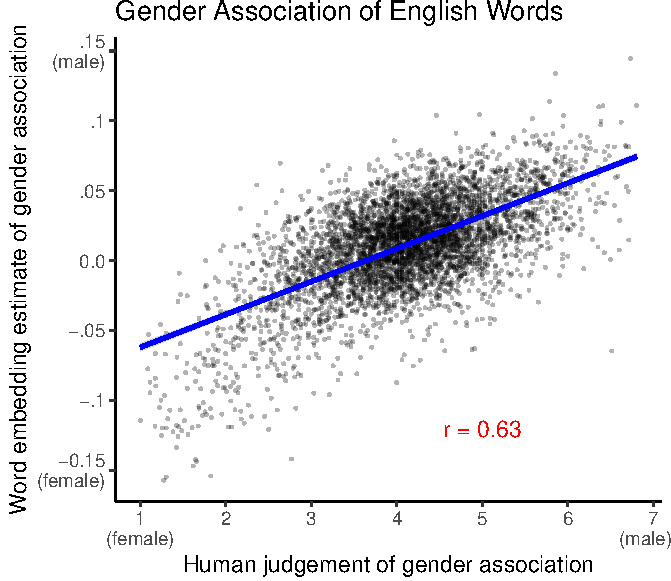
\includegraphics{iat_lang_files/figure-latex/unnamed-chunk-11-1.pdf}
\caption{\label{fig:unnamed-chunk-11}Word embedding estimates of gender bias
as a function of human judgments of gender bias (Study 1a). Each point
corresponds to a word. Larger numbers indicate stronger association with
males. Blue line shows linear fit and the error band corresponds to a
standard error (too small to be visible).}
\end{figure}

\subsection{Study 1b: Gender bias across
languages}\label{study-1b-gender-bias-across-languages}

Having validated our method, we next turn toward examining the
relationship between psychological and linguistic gender biases. In
Study 1b, we estimate the magnitude of the gender-career bias in the
dominant language spoken in the countries of the Project Implicit
participants and compare it with estimates of behavioral gender bias
from the Project Implicit data set.

\subsubsection{Methods}\label{methods-1}

For each country represented in our analysis of the Project Implicit, we
identified the most frequently spoken language in each country using
Ethnologue (Simons \& (eds.)., 2018). This included a total of 27 unique
languages. For two languages, Zulu and Tagalog, the corpora that the
models were trained on (see below) were too small to be reliable, and so
we excluded these languages from our analysis. Our final sample included
25 languages, representing XX different language families.

For each language, we then obtained translations from native speakers
for the stimuli in the Project Implicit gender-career IAT behavioral
task (Nosek et al., 2002) with one slight modification. In the
behavioral task, proper names were used to cue the male and female
categories (e.g.~\enquote{John,} \enquote{Amy}), but because there are
not direct translation equivalents of proper names, we instead used a
set of generic gendered words which had been previously used for a
different version of the gender IAT (e.g., ``man,'' ``woman;'' Nosek et
al., 2002). Our linguistic stimuli were therefore a set of 8 female and
8 male Target Words (identical to Study 1a), a set of 8 Attribute Words
associated with the concept \enquote{career} (\enquote{career,}
\enquote{executive,} \enquote{management,} \enquote{professional,}
\enquote{corporation,} \enquote{salary,} \enquote{office,}
\enquote{business}) and 8 Attribute Words associated with the concept
\enquote{family} (\enquote{family,} \enquote{home,} \enquote{parents,}
\enquote{children,} \enquote{cousins,} \enquote{marriage,}
\enquote{wedding,} \enquote{relatives}).

We used these translations to calculate a gender bias effect size from
word embedding models trained on text in each language. Our effect size
measure is a standardized difference score of the relative similarity of
the target words to the target attributes (i.e.~relative similarity of
male to career vs.~relative similarity of female to career). Our effect
size measure is identical to that used by CBN with one exception (see SM
for replication of CBN on our corpora). Namely, for languages with
grammatically gendered Attribute Words (e.g., ninas for female children
in Spanish), we calculated the relationship between target words and
attribute words of the same gender (i.e. \enquote{hombre} (man) to
\enquote{ninos} and \enquote{mujer} (woman) to \enquote{ninas}). In
cases where there were multiple translations for a word, or the
translation contained multiple words, we averaged across words such that
each of our target words was associated with a single vector in each
language. Our effect size measure is analogous to the to the behavioral
effect size measure obtained from the IAT task in Project Implicit,
where larger values indicate larger gender bias.

We calculated gender bias estimates based on models trained on two
different corpora: Wikipedia (Bojanowski et al., 2016) and Subtitles
{[}where are these from?{]}. These two models capture different types of
XX. We then compared the effect size of the linguistic gender bias to
the behavioral IAT gender bias estimated from Project Implicit,
averaging across countries that speak whose participants speak the same
language.

\subsubsection{Results}\label{results}

\begin{figure}
\centering
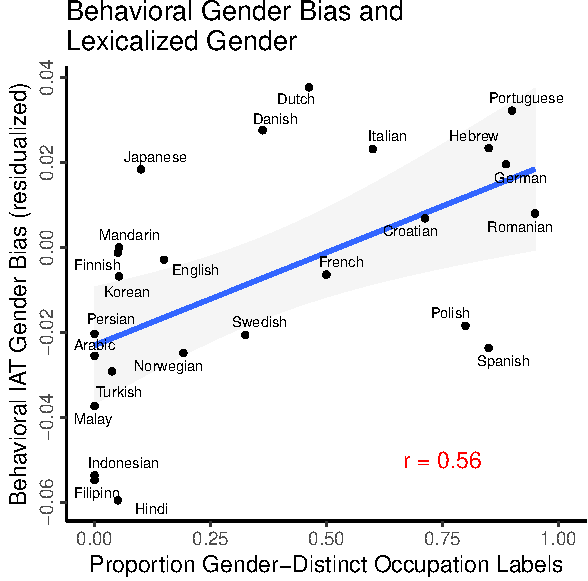
\includegraphics{iat_lang_files/figure-latex/unnamed-chunk-14-1.pdf}
\caption{\label{fig:unnamed-chunk-14}Residualized behavioral IAT gender bias
as a function of linguistic gender bias, with each point corresponding
to a language (Study 1b). Linguistic biases are estimated from models
trained on each language using a subtitle corpus (left) and a sample of
Wikipedia (right). Larger values indicate a larger bias to associate men
with the concept of career and women with the concept of family. Error
bands indicate standard error of the model estimate.}
\end{figure}

The estimate of gender bias for each language was positively correlated
the implicit gender bias of participants from countries where that
language was dominant (and, we assume, was the native language of most
of these individuals; \emph{r} = 0.36; \emph{p} = 0.08; Fig. 2). This
relationship held when controlling for median country age in a linear
model (\(\beta\)= 0.02; \emph{SE} = 0.01, \emph{p} = 0.09). Linguistic
gender bias was not correlated with explicit gender bias (\emph{r} =
0.29; \emph{p} = 0.16). {[}Percentage women in stem and language are
marginal p = .06{]}. Table 1 shows the language-level correlations
between all variables.

\begin{table}

\caption{\label{tab:corrtable}Correlation (Pearson's r) for all measures in Study 1 at the level of languages. Asterisks indicate significance at the .05 level.}
\centering
\fontsize{10}{12}\selectfont
\begin{tabular}[t]{l>{\raggedleft\arraybackslash}p{2.5cm}>{\raggedleft\arraybackslash}p{2.5cm}>{\raggedleft\arraybackslash}p{2.5cm}>{\raggedleft\arraybackslash}p{2.5cm}lrrrrlrrrrlrrrrlrrrr}
\toprule
 & Linguistic Gender Bias 
(Subtitles) & Linguistic Gender Bias 
 (Wikipedia) & Explicit Gender Bias 
 (residualized) & Behavioral Gender Bias (residualized IAT score)\\
\midrule
Language IAT (Subtitles) &  &  &  & \\
Language IAT (Wikipedia) & .58** &  &  & \\
Residualized Explicit Bias & .04 & .29 &  & \\
Residualized Behavioral IAT & .42 & .36 & .14 & \\
Percent Women in Stem & -.40 & -.19 & .30 & -.44\\
\bottomrule
\end{tabular}
\end{table}

\subsubsection{Discussion}\label{discussion}

\section{Study 2: Gender bias and
grammar}\label{study-2-gender-bias-and-grammar}

The findings in Study 1 are consistent with the possibility that
people's implicit biases are in part caused by input from language
(language-as-causal) and that the linguistic biases simply reflect
existing biases (language-as-reflection). In Study 2, we try to
distinguish between the two possibilities by examining whether
linguistic biases are associated with grammatical gender, a structural
aspect of language that is clearly not caused by people's gender biases.
{[}Describe what grammatical gender is{]}. We predicted that grammatical
gender would act to exaggerate the linguistic biases present in the
language. To the extent that these are causally related to people's
implicit biases, these languages may be providing their speakers with
additional exposure to gender biases thereby increasing their speakers'
implicit biases.

\subsubsection{Method}\label{method}

We coded each of the languages in our sample (Study 1) for grammatical
gender. We used a coarse binary coding scheme, categorizing a language
as encoding grammatical gender if it made any gender distinction on noun
classes (masculine, feminine, common or neuter), and as not encoding
gender grammatically otherwise.

\subsubsection{Results and Discussion}\label{results-and-discussion-1}

\begin{figure}
\centering
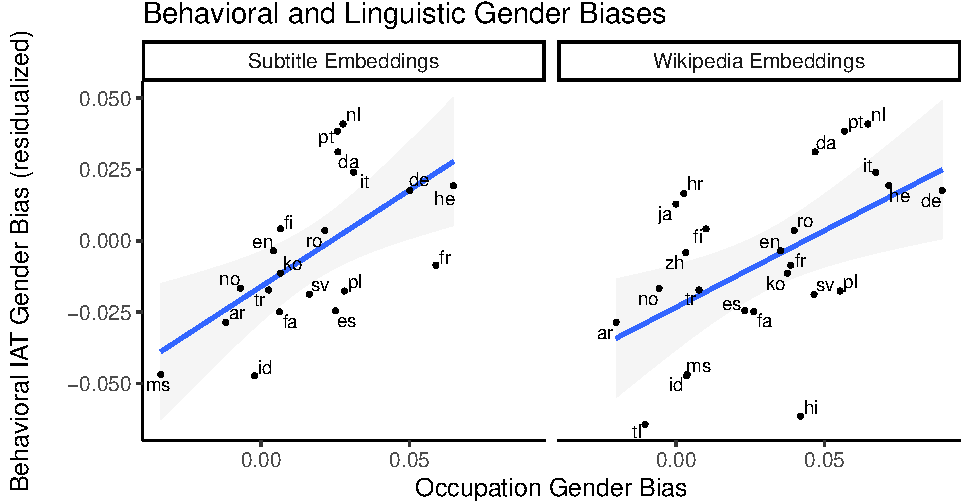
\includegraphics{iat_lang_files/figure-latex/unnamed-chunk-19-1.pdf}
\caption{\label{fig:unnamed-chunk-19}Residualized behavioral IAT gender bias
as a function of whether or not the language encodes grammatical gender.
Each label code corresponds to a language. The bold vertical line
corresponds to the group median, and the box width indicates the first
and third quartile.}
\end{figure}

\section{General Discussion}\label{general-discussion}

\newpage

\section{References}\label{references}

\begingroup
\setlength{\parindent}{-0.5in} \setlength{\leftskip}{0.5in}

\hypertarget{refs}{}
\hypertarget{ref-bian2017gender}{}
Bian, L., Leslie, S.-J., \& Cimpian, A. (2017). Gender stereotypes about
intellectual ability emerge early and influence children's interests.
\emph{Science}, \emph{355}(6323), 389--391.

\hypertarget{ref-bojanowski2016enriching}{}
Bojanowski, P., Grave, E., Joulin, A., \& Mikolov, T. (2016). Enriching
word vectors with subword information.

\hypertarget{ref-caliskan2017semantics}{}
Caliskan, A., Bryson, J. J., \& Narayanan, A. (2017). Semantics derived
automatically from language corpora contain human-like biases.
\emph{Science}, \emph{356}(6334), 183--186.

\hypertarget{ref-ceci2011understanding}{}
Ceci, S. J., \& Williams, W. M. (2011). Understanding current causes of
women's underrepresentation in science. \emph{Proceedings of the
National Academy of Sciences}, 201014871.

\hypertarget{ref-ciafactbook}{}
Central Intelligence Agency (CIA). (2017). The World Factbook. Retrieved
from
\url{https://www.cia.gov/library/publications/the-world-factbook/index.html}

\hypertarget{ref-cimpian2011generic}{}
Cimpian, A., \& Markman, E. M. (2011). The generic/nongeneric
distinction influences how children interpret new information about
social others. \emph{Child Development}, \emph{82}(2), 471--492.

\hypertarget{ref-cimpian2012good}{}
Cimpian, A., Mu, Y., \& Erickson, L. C. (2012). Who is good at this
game? Linking an activity to a social category undermines children's
achievement. \emph{Psychological Science}, \emph{23}(5), 533--541.

\hypertarget{ref-corbett1991}{}
Corbett, G. G. (1991). \emph{Gender}. Cambridge: Cambridge University
Press.

\hypertarget{ref-epi}{}
\emph{EF English Proficiency Index}. (2017). Retrieved from
\url{https://www.ef.edu/epi/}

\hypertarget{ref-firth1957synopsis}{}
Firth, J. (1957). A synopsis of linguistic theory 1930-1955 in studies
in linguistic analysis, philological society. Oxford.

\hypertarget{ref-forscher2016meta}{}
Forscher, P. S., Lai, C., Axt, J., Ebersole, C. R., Herman, M., Devine,
P. G., \& Nosek, B. A. (2016). A meta-analysis of change in implicit
bias.

\hypertarget{ref-gelman2004mother}{}
Gelman, S. A., Taylor, M. G., Nguyen, S. P., Leaper, C., \& Bigler, R.
S. (2004). Mother-child conversations about gender: Understanding the
acquisition of essentialist beliefs. \emph{Monographs of the Society for
Research in Child Development}, i--142.

\hypertarget{ref-greenwald1998measuring}{}
Greenwald, A. G., McGhee, D. E., \& Schwartz, J. L. (1998). Measuring
individual differences in implicit cognition: The implicit association
test. \emph{Journal of Personality and Social Psychology}, \emph{74}(6),
1464.

\hypertarget{ref-greenwald2003understanding}{}
Greenwald, A. G., Nosek, B. A., \& Banaji, M. R. (2003). Understanding
and using the Implicit Association Test: An improved scoring algorithm.
\emph{Journal of Personality and Social Psychology}, \emph{85}(2), 197.

\hypertarget{ref-joulin2016bag}{}
Joulin, A., Grave, E., Bojanowski, P., \& Mikolov, T. (2016). Bag of
tricks for efficient text classification. \emph{arXiv Preprint
arXiv:1607.01759}.

\hypertarget{ref-leslie2015expectations}{}
Leslie, S.-J., Cimpian, A., Meyer, M., \& Freeland, E. (2015).
Expectations of brilliance underlie gender distributions across academic
disciplines. \emph{Science}, \emph{347}(6219), 262--265.

\hypertarget{ref-mikolov2013efficient}{}
Mikolov, T., Chen, K., Corrado, G., \& Dean, J. (2013). Efficient
estimation of word representations in vector space.

\hypertarget{ref-miller2015women}{}
Miller, D. I., Eagly, A. H., \& Linn, M. C. (2015). Women's
representation in science predicts national gender-science stereotypes:
Evidence from 66 nations. \emph{Journal of Educational Psychology},
\emph{107}(3), 631.

\hypertarget{ref-nosek2002harvesting}{}
Nosek, B. A., Banaji, M. R., \& Greenwald, A. G. (2002). Harvesting
implicit group attitudes and beliefs from a demonstration web site.
\emph{Group Dynamics: Theory, Research, and Practice}, \emph{6}(1), 101.

\hypertarget{ref-phillips2003can}{}
Phillips, W., \& Boroditsky, L. (2003). Can quirks of grammar affect the
way you think? Grammatical gender and object concepts. In
\emph{Proceedings of the 25th Annual Meeting of the Cognitive Science
Society} (pp. 928--933).

\hypertarget{ref-rhodes2008preschoolers}{}
Rhodes, M., \& Brickman, D. (2008). Preschoolers' responses to social
comparisons involving relative failure. \emph{Psychological Science},
\emph{19}(10), 968--972.

\hypertarget{ref-scott2018glasgow}{}
Scott, G. G., Keitel, A., Becirspahic, M., Yao, B., \& Sereno, S. C.
(2018). The glasgow norms: Ratings of 5,500 words on nine scales.
\emph{Behavior Research Methods}, 1--13.

\hypertarget{ref-sera1994grammatical}{}
Sera, M. D., Berge, C. A., \& Castillo Pintado, J. del. (1994).
Grammatical and conceptual forces in the attribution of gender by
English and Spanish speakers. \emph{Cognitive Development}, \emph{9}(3),
261--292.

\hypertarget{ref-simons2018}{}
Simons, G. F., \& (eds.)., C. D. F. (Eds.). (2018). Ethnologue:
Languages of the world. \emph{Ethnologue: Languages of the World}.

\hypertarget{ref-stoet2018gender}{}
Stoet, G., \& Geary, D. C. (2018). The gender-equality paradox in
science, technology, engineering, and mathematics education.
\emph{Psychological Science}, \emph{29}(4), 581--593.

\hypertarget{ref-whorf1945grammatical}{}
Whorf, B. (1945). Grammatical categories. \emph{Language}, 1--11.

\hypertarget{ref-wps}{}
Women, Peace and Security Index. (2017). Retrieved from
\url{https://giwps.georgetown.edu/}

\endgroup


\end{document}
